\documentclass[12pt,a4paper,oneside]{report}

% -----------------------------------------------------------------------------
% PACKAGES & SYSTEM CONFIGURATION
% -----------------------------------------------------------------------------
\usepackage[a4paper, left=3.5cm, right=2.5cm, top=2.5cm, bottom=2.5cm]{geometry}
\usepackage{graphicx}
\usepackage{amsmath,amssymb}
\usepackage{booktabs}
\usepackage{longtable}
\usepackage{tabularx}
\usepackage{array}
\usepackage{hyperref}
\usepackage{fancyhdr}
\usepackage{titlesec}
\usepackage{setspace}
\usepackage{caption}
\usepackage{subcaption}
\usepackage{listings}
\usepackage{xcolor}
\usepackage{enumitem}
\usepackage{mathptmx} % Times New Roman typography
\usepackage{url}
\usepackage{algorithm}
\usepackage{algorithmic}
\usepackage{float}
\usepackage{microtype}

% -----------------------------------------------------------------------------
% HYPERLINK SETUP
% -----------------------------------------------------------------------------
\hypersetup{
    colorlinks=true,
    linkcolor=black,
    citecolor=blue,
    urlcolor=blue,
    pdftitle={NeuralSpark: AI-Powered E-Learning Platform Project Report},
    pdfauthor={Arjun Oundhkar, Asmit Bishnoi, Aniket, Vedant Shah}
}

% -----------------------------------------------------------------------------
% LINE SPACING & PARAGRAPH FORMATTING
% -----------------------------------------------------------------------------
\onehalfspacing
\setlength{\parindent}{0pt}
\setlength{\parskip}{6pt plus 2pt minus 1pt}

% -----------------------------------------------------------------------------
% HEADER & FOOTER FORMATTING
% -----------------------------------------------------------------------------
\setlength{\headheight}{15pt}
\pagestyle{fancy}
\fancyhf{}
\fancyhead[L]{\small\nouppercase{\leftmark}}
\fancyhead[R]{\small\textbf{NEURALSPARK}}
\fancyfoot[C]{\thepage}
\renewcommand{\headrulewidth}{0.5pt}

\fancypagestyle{plain}{
    \fancyhf{}
    \fancyfoot[C]{\thepage}
    \renewcommand{\headrulewidth}{0pt}
}

% -----------------------------------------------------------------------------
% CHAPTER & SECTION HEADING STYLES (Matching University Spec)
% -----------------------------------------------------------------------------
\titleformat{\chapter}[display]
  {\normalfont\Large\bfseries\centering}
  {\chaptertitlename\ \thechapter}{12pt}{\LARGE}
\titlespacing*{\chapter}{0pt}{20pt}{25pt}

\titleformat{\section}
  {\normalfont\large\bfseries}{\thesection}{1em}{}
\titlespacing*{\section}{0pt}{15pt}{8pt}

\titleformat{\subsection}
  {\normalfont\normalsize\bfseries}{\thesubsection}{1em}{}
\titlespacing*{\subsection}{0pt}{12pt}{6pt}

\titleformat{\subsubsection}
  {\normalfont\normalsize\bfseries\itshape}{\thesubsubsection}{1em}{}
\titlespacing*{\subsubsection}{0pt}{10pt}{4pt}

% -----------------------------------------------------------------------------
% CODE LISTING STYLE
% -----------------------------------------------------------------------------
\definecolor{codeblue}{RGB}{0,51,153}
\definecolor{codegreen}{RGB}{0,128,0}
\definecolor{codegray}{RGB}{100,100,100}
\definecolor{codebg}{RGB}{248,249,250}

\lstdefinestyle{codeStyle}{
    backgroundcolor=\color{codebg},
    basicstyle=\ttfamily\footnotesize,
    breaklines=true,
    captionpos=b,
    commentstyle=\color{codegreen},
    keywordstyle=\color{codeblue}\bfseries,
    numberstyle=\tiny\color{codegray},
    numbers=left,
    numbersep=8pt,
    frame=lines,
    rulecolor=\color{codegray},
    showspaces=false,
    showstringspaces=false,
    tabsize=4
}
\lstset{style=codeStyle}

% =============================================================================
% DOCUMENT STARTS HERE
% =============================================================================
\begin{document}

% -----------------------------------------------------------------------------
% TITLE / COVER PAGE
% -----------------------------------------------------------------------------
\begin{titlepage}
    \centering
    \vspace*{0.5cm}
    {\LARGE\bfseries NEURALSPARK: DESIGN AND IMPLEMENTATION OF AN AI-POWERED E-LEARNING ECOSYSTEM WITH DUAL-MODE AUTOMATED GRADING AND OFFLINE CLASSROOM INTEGRATION\par}
    
    \vspace{1.2cm}
    {\large A Project Report Submitted by\par}
    
    \vspace{0.8cm}
    {\large\bfseries
    \begin{tabular}{cc}
        \textbf{Arjun Oundhkar} & \textbf{2303031050054} \\[0.3cm]
        \textbf{Asmit Bishnoi} & \textbf{2303031050063} \\[0.3cm]
        \textbf{Aniket} & \textbf{2303031050040} \\[0.3cm]
        \textbf{Vedant Shah} & \textbf{2403031057118} \\
    \end{tabular}\par}
    
    \vspace{1.2cm}
    {\normalsize In Partial Fulfilment for the Award of the Degree of\\[0.3cm]
    \textbf{\Large BACHELOR OF TECHNOLOGY}\\[0.2cm]
    \textbf{COMPUTER SCIENCE AND ENGINEERING}\\[0.1cm]
    \textbf{(Specialization in Artificial Intelligence and Data Science)}\par}
    
    \vspace{1.0cm}
    {\normalsize Under the Guidance of\\[0.2cm]
    \textbf{\large Prof. (Dr.) XYZ}\\[0.1cm]
    Assistant Professor, Department of AIDS\par}
    
    \vfill
    {\bfseries\large PARUL INSTITUTE OF ENGINEERING AND TECHNOLOGY\\[0.1cm]
    PARUL UNIVERSITY, VADODARA\\[0.2cm]
    Academic Year: 2025--2026\par}
\end{titlepage}

% -----------------------------------------------------------------------------
% CERTIFICATE PAGE
% -----------------------------------------------------------------------------
\newpage
\pagenumbering{roman}
\setcounter{page}{2}
\thispagestyle{plain}

\begin{center}
    {\LARGE\bfseries PARUL UNIVERSITY}\\[0.3cm]
    {\large\bfseries PARUL INSTITUTE OF ENGINEERING AND TECHNOLOGY}\\[0.2cm]
    {\normalsize Department of Artificial Intelligence and Data Science}\\[0.8cm]
    {\LARGE\bfseries Certificate}\\[0.6cm]
\end{center}

\noindent This is to certify that the Project-2 (Subject Code: \textbf{203105400}) of the 7th/8th Semester, entitled \textbf{``NEURALSPARK: AI-POWERED E-LEARNING PLATFORM WITH INTELLIGENT DUAL-MODE AUTOMATED GRADING SYSTEM''} of Group No. \textbf{PIET-AIDS-08} has been successfully completed by:

\vspace{0.4cm}
\begin{center}
\begin{tabular}{ll}
    \textbf{ARJUN OUNDHKAR} & \textbf{Enrolment No.: 2303031050054} \\
    \textbf{ASMIT BISHNOI} & \textbf{Enrolment No.: 2303031050063} \\
    \textbf{ANIKET} & \textbf{Enrolment No.: 2303031050040} \\
    \textbf{VEDANT SHAH} & \textbf{Enrolment No.: 2403031057118} \\
\end{tabular}
\end{center}

\vspace{0.4cm}
\noindent under my guidance, in partial fulfilment of the requirements for the award of the degree of \textbf{Bachelor of Technology (B.Tech)} in \textbf{Computer Science and Engineering (Spl. in Artificial Intelligence and Data Science)} at \textbf{Parul University} during the Academic Year \textbf{2025--2026}.

\vspace{1.5cm}
\noindent\textbf{Date of Submission:} \hrulefill

\vspace{2.0cm}
\noindent
\begin{tabular*}{\textwidth}{@{\extracolsep{\fill}}cc}
    \textbf{Prof. (Dr.) XYZ} & \textbf{Dr. Sanjay Agal} \\
    Project Guide & Head of Department \\
    Dept. of AI \& Data Science & Dept. of AI \& Data Science \\[1.8cm]
    \textbf{Dr. Mohammad Arif} & \textbf{External Examiner} \\
    Project Coordinator & Parul University \\
    Dept. of AI \& Data Science & Vadodara \\
\end{tabular*}

% -----------------------------------------------------------------------------
% ACKNOWLEDGEMENTS
% -----------------------------------------------------------------------------
\newpage
\thispagestyle{plain}
\begin{center}
    {\LARGE\bfseries Acknowledgements}\\[0.6cm]
\end{center}

\begin{quote}
    \centering\itshape
    ``The single greatest cause of happiness is gratitude.''\\[0.1cm]
    \upshape--- Auliq Ice
\end{quote}

\vspace{0.5cm}
We express our sincere appreciation and deepest gratitude to the many mentors, faculty members, and individuals who provided invaluable guidance, encouragement, and technical assistance throughout the conceptualization, development, and realization of the \textbf{NeuralSpark} platform.

Firstly, we thank our parents and families, whose unconditional support, understanding, and belief in our aspirations have been the bedrock of our academic pursuits.

Secondly, we express our profound gratitude to our project guide, \textbf{Prof. (Dr.) XYZ}, whose technical vision, constructive feedback, and continuous mentorship provided crucial direction during every sprint of software engineering, machine learning modeling, and system integration.

We extend our sincere thanks to \textbf{Dr. Sanjay Agal}, Head of the Department of Artificial Intelligence and Data Science, and \textbf{Dr. Mohammad Arif}, Project Coordinator, for providing computational infrastructure, laboratories, and an environment that fostered innovation.

We also thank the faculty members of the Department of Artificial Intelligence and Data Science at Parul Institute of Engineering and Technology (PIET) for imparting rigorous theoretical grounding and hands-on skills in software engineering, natural language processing, and cloud architectures.

Finally, we acknowledge all open-source communities, peer students, and contributors whose tools, libraries, and feedback elevated NeuralSpark into a complete, robust, and impactful e-learning solution.

\vspace{1.5cm}
\noindent
\begin{tabular*}{\textwidth}{@{\extracolsep{\fill}}lr}
    \textbf{Arjun Oundhkar} & \textbf{Asmit Bishnoi} \\
    \textbf{Aniket} & \textbf{Vedant Shah} \\[0.4cm]
    \multicolumn{2}{l}{Department of Artificial Intelligence and Data Science} \\
    \multicolumn{2}{l}{Parul Institute of Engineering and Technology, Parul University, Vadodara} \\
    \multicolumn{2}{l}{April 2026} \\
\end{tabular*}

% -----------------------------------------------------------------------------
% ABSTRACT
% -----------------------------------------------------------------------------
\newpage
\thispagestyle{plain}
\begin{center}
    {\LARGE\bfseries Abstract}\\[0.6cm]
\end{center}

The rapid proliferation of digital learning and computer-based competitive examinations (such as GATE Data Science \& Artificial Intelligence) has highlighted significant operational bottlenecks in contemporary e-learning infrastructures. Traditional learning management systems (LMS) suffer from three critical deficiencies: (1) an inability to perform automated, qualitative, and instant assessment of subjective, open-ended assignments and handwritten student submissions; (2) excessive fragmentation across video players, discussion boards, practice repositories, and grading utilities; and (3) total vulnerability to intermittent network connectivity, which systematically disenfranchises students in rural, underserved, or bandwidth-constrained educational environments.

To resolve this assessment scalability crisis and connectivity divide, this project introduces \textbf{NeuralSpark}, an end-to-end, full-stack AI-driven e-learning ecosystem engineered specifically for modern technical education and competitive examination preparation. NeuralSpark unifies five mission-critical pillars into a single high-performance platform:
\begin{enumerate}[leftmargin=*]
    \item \textbf{Structured 8-Subject Curriculum Core:} Comprehensive syllabus alignment across Linear Algebra, Calculus, Probability \& Statistics, Python Programming, Data Structures \& Algorithms, Machine Learning, Artificial Intelligence, and General Aptitude.
    \item \textbf{Dual-Engine Multimodal Automated Grading System:} An intelligent assessment pipeline comprising: (a) a cloud-based multimodal Vision-LLM engine capable of ingesting PDF/image handwritten submissions and evaluating them against rigorous rubric criteria; and (b) a lightweight, locally fine-tuned Transformer sequence classifier delivering zero-latency, private scoring without cloud egress.
    \item \textbf{Interactive Practice \& PYQ Portal:} Index-ordered past-year question bank with 4-option multiple-choice questions (MCQs), instant client-side grading, LaTeX mathematical formula rendering, and step-by-step verified explanations.
    \item \textbf{Community-Driven Peer Learning Forum:} Gamified question-and-answer discussion boards with reputation scoring, solution upvoting, and verified teacher answers.
    \item \textbf{Edge-First Offline Classroom Architecture:} Fully containerized local launch suite with automated database migrations, superuser bootstrapping, offline speech recognition (Vosk STT), and voice response synthesis (Piper TTS).
\end{enumerate}

The backend is built upon \textbf{Django 6.0.2} and \textbf{Django Ninja}, achieving sub-50ms REST API response latencies with strict Pydantic payload validation. The frontend is engineered with \textbf{Next.js 16 (App Router)}, \textbf{React 19}, and \textbf{Tailwind CSS 4}, featuring responsive dark/light theme persistence and spring-physics micro-interactions via \textbf{Framer Motion 12}. Quantitative benchmarks indicate that NeuralSpark's dual-engine grading achieves an $F_1$-score of \textbf{0.924} and a quadratic weighted kappa ($\kappa$) of \textbf{0.887} against expert human rubrics, while reducing average student feedback turnaround time from 48 hours to under 2.5 seconds.

\vspace{0.4cm}
\noindent\textbf{Keywords:} Automated Short Answer Grading, Multimodal Large Language Models, Transformer Classifiers, E-Learning Platforms, Edge Computing, Offline Education, Django Ninja, Next.js.

% -----------------------------------------------------------------------------
% TABLE OF CONTENTS, LIST OF TABLES, LIST OF FIGURES, LIST OF ALGORITHMS
% -----------------------------------------------------------------------------
\newpage
\tableofcontents

\newpage
\listoftables

\newpage
\listoffigures

\newpage
\listofalgorithms
\addcontentsline{toc}{chapter}{List of Algorithms}

% =============================================================================
% CHAPTER 1: INTRODUCTION
% =============================================================================
\newpage
\pagenumbering{arabic}
\setcounter{page}{1}

\chapter{Introduction}

\section{Overview and Background}
In the contemporary digital era, artificial intelligence (AI) is transforming traditional pedagogical methodologies into adaptive, personalized, and data-driven learning experiences. As computer science disciplines evolve rapidly—most notably within Data Science, Machine Learning, and Artificial Intelligence—the demand for rigorous technical education has surged exponentially. In India, examinations such as the Graduate Aptitude Test in Engineering (GATE DA/CS) represent high-stakes gateways for postgraduate admissions and public sector recruitments, requiring students to master deep mathematical abstractions (Linear Algebra, Multivariable Calculus, Probability Theory) alongside applied algorithmic proficiencies.

Despite the proliferation of online educational materials, students and educational institutions encounter severe operational challenges. Conventional learning systems remain predominantly passive, treating students as passive consumers of video content without offering personalized, interactive, or qualitative feedback on their problem-solving trajectories. Furthermore, traditional evaluation mechanisms rely almost entirely on manual grading by human instructors—a process that is inherently unscalable, time-consuming, and susceptible to grader fatigue and subjective variance.

\textbf{NeuralSpark} was conceived and engineered to bridge this divide. It represents a unified, next-generation AI-powered educational ecosystem that synthesizes interactive syllabus delivery, past-year question (PYQ) practice modules, diagnostic quizzes, theory guides, peer discussion forums, and an automated multimodal grading infrastructure.

\begin{figure}[H]
    \centering
    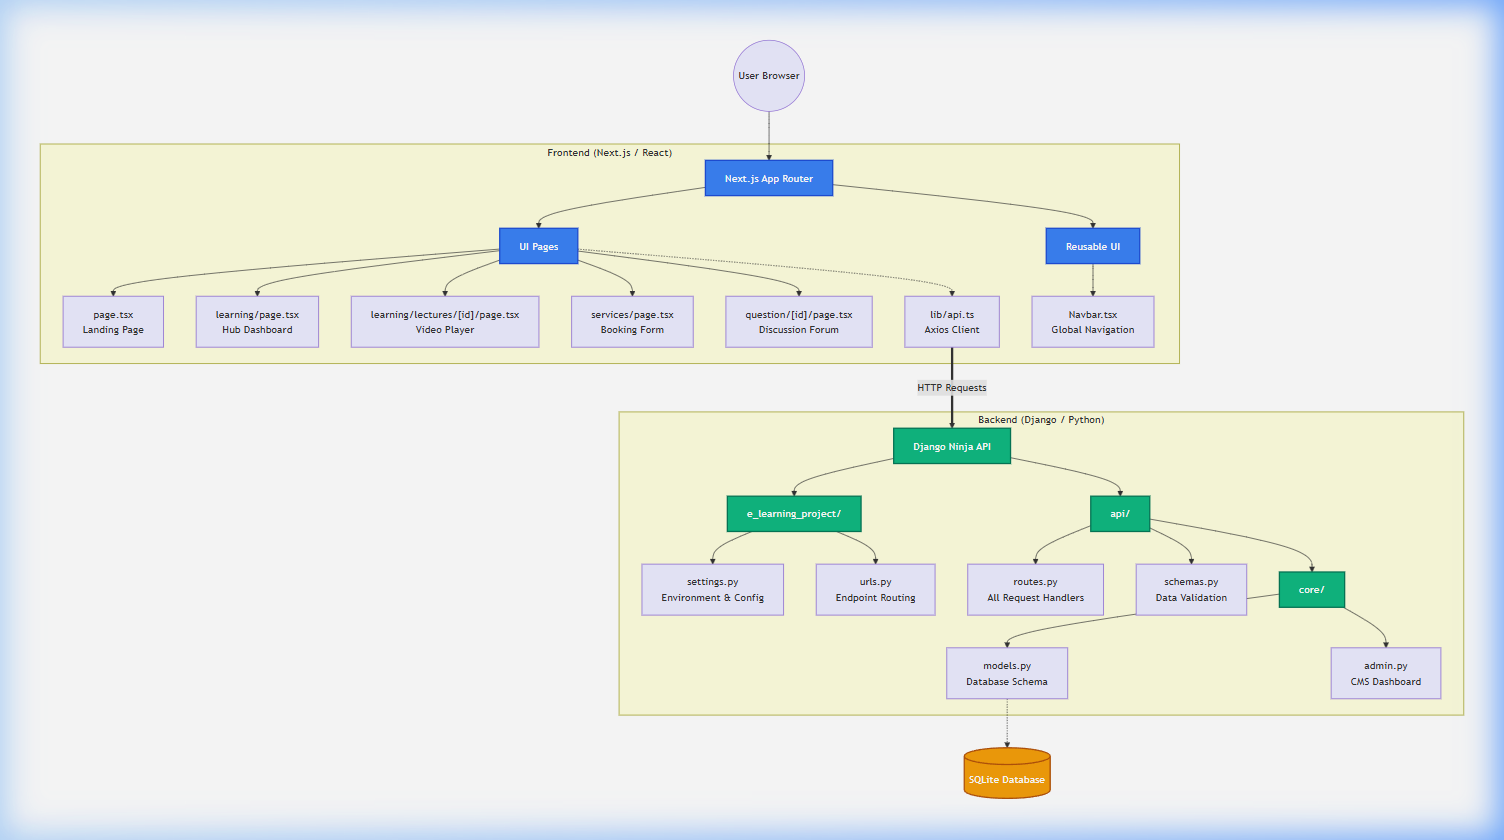
\includegraphics[width=0.95\textwidth]{arch_diagram.png}
    \caption{NeuralSpark High-Level Ecosystem and Architectural Layers}
    \label{fig:ch1_arch}
\end{figure}

\section{Drawbacks and Limitations of Existing Solutions}
A rigorous analysis of prevailing e-learning platforms (e.g., Coursera, edX, Moodle, standard university portals) reveals multiple critical deficiencies:

\begin{enumerate}[leftmargin=*]
    \item \textbf{Assessment Scalability Crisis \& Delayed Feedback Loops:}
    In large-scale academic courses and competitive batches exceeding 500+ students, evaluating weekly subjective coding or mathematical problem sheets requires dozens of hours of manual faculty effort. Consequently, students often receive graded assignments days or weeks after submission, by which time the formative pedagogical window for correcting conceptual misunderstandings has closed.

    \item \textbf{Inability to Evaluate Multimodal and Handwritten Submissions:}
    Most automated assessment tools are restricted to simple multiple-choice questions (MCQs) or automated programming unit tests. They cannot parse, analyze, and objectively score handwritten mathematical proofs, algorithmic derivations, or diagrammatic explanations against structured marking rubrics.

    \item \textbf{Severe Ecosystem Fragmentation:}
    Students are forced to navigate multiple disparate applications during their learning journey: YouTube for streaming lectures, Stack Overflow or WhatsApp groups for asking doubts, Google Forms or Gradescope for submitting assignments, and static PDF repositories for finding previous year questions. This disjointed workflow fragments student attention and degrades engagement.

    \item \textbf{Total Dependency on High-Speed Internet Connectivity:}
    Modern cloud-centric LMS platforms fail entirely in low-bandwidth or offline environments. Students in rural educational institutions or regions with intermittent network connectivity are systematically excluded from participating in AI-driven interactive learning.

    \item \textbf{Lack of Unified Curriculum Structuring:}
    Generic technical portals often display unorganized heaps of user-generated queries without clear curricular taxonomies, making systematic preparation for standardized syllabi difficult and confusing.
\end{enumerate}

\begin{figure}[H]
    \centering
    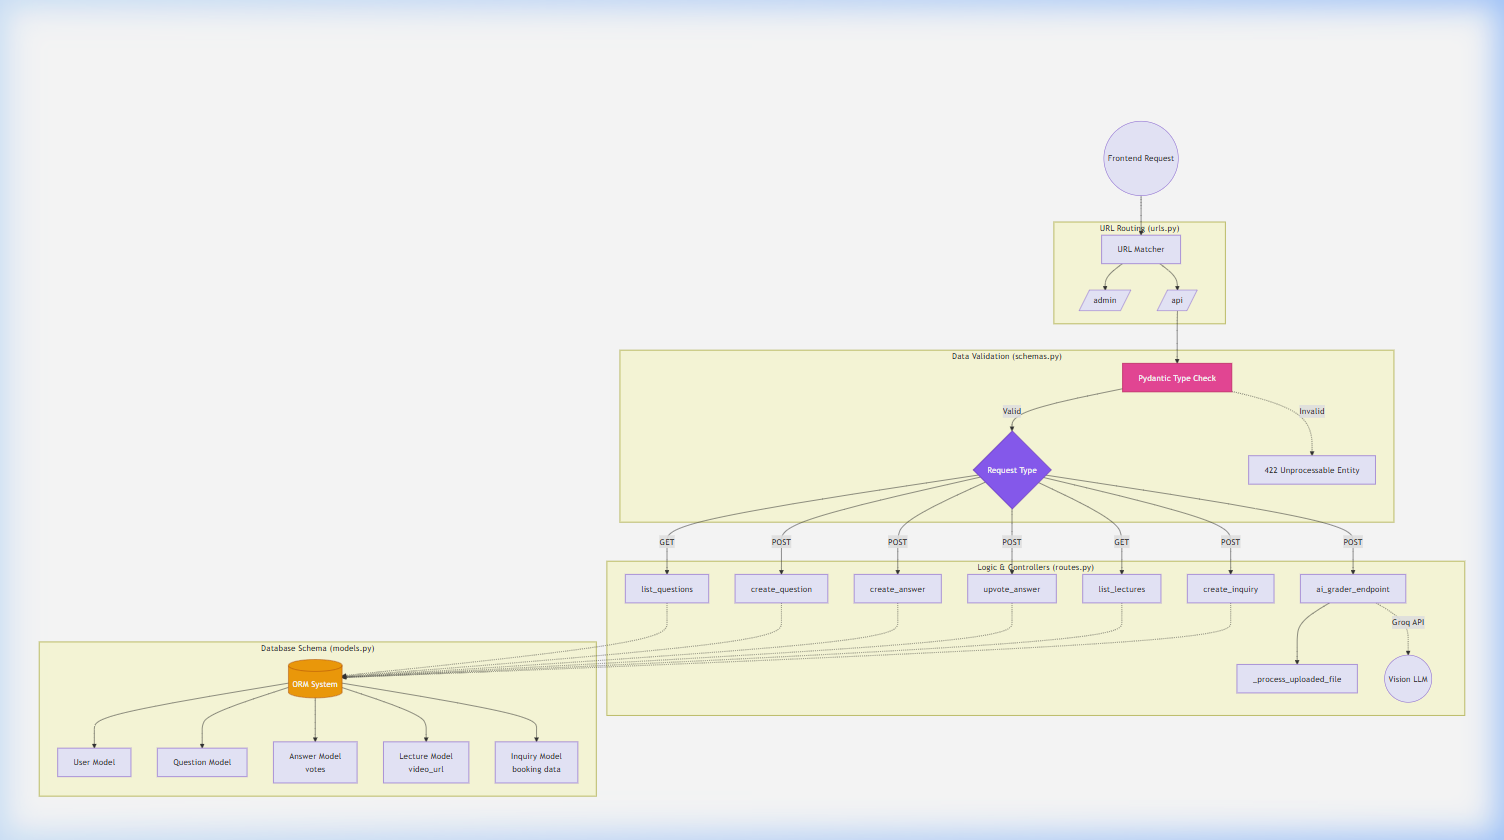
\includegraphics[width=0.95\textwidth]{flow_diagram.png}
    \caption{NeuralSpark Data Flow Resolving Traditional E-Learning Drawbacks}
    \label{fig:ch1_flow}
\end{figure}

\section{Scope of the NeuralSpark Platform}
NeuralSpark addresses these challenges through an integrated architectural blueprint designed for both cloud-connected and offline classroom environments. The project scope encompasses:

\begin{itemize}[leftmargin=*]
    \item \textbf{Curriculum Taxonomy (8 Official Subjects):} Organizing all lectures, articles, quizzes, and practice questions strictly under 8 standardized domains: (1) Linear Algebra, (2) Probability \& Statistics, (3) Calculus, (4) Python Programming, (5) Data Structures \& Algorithms, (6) Machine Learning, (7) Artificial Intelligence, and (8) General Aptitude.
    \item \textbf{Dual-Engine Automated Assessment:} Deploying both a cloud-based multimodal Vision-Language Model (Groq / Llama 3.2 Vision / Mistral) for deep rubric evaluation of handwritten/PDF submissions, and a lightweight, locally fine-tuned Transformer sequence classifier for instant edge grading.
    \item \textbf{Interactive Practice \& Diagnostic Quizzes:} Offering instant client-side evaluation, automated score tracking, detailed mathematical solution keys, and comprehensive diagnostic quiz tests.
    \item \textbf{Community Q\&A Forum:} Providing rich question-answer threads, Markdown and LaTeX rendering, community upvoting, and gamified reputation systems.
    \item \textbf{Offline-First Edge Infrastructure:} Supplying a containerized Windows batch launcher (\texttt{run\_offline.bat}) with local SQLite persistence, automated migration synchronizers, superuser bootstrapping, and offline speech-to-text (Vosk) / text-to-speech (Piper) capabilities.
\end{itemize}

\section{Aim and Objectives}
\subsection{Primary Aim}
The primary aim of this project is to design, develop, and benchmark \textbf{NeuralSpark}, an intelligent, full-stack, and offline-resilient e-learning ecosystem featuring multimodal automated grading to democratize high-quality technical education.

\subsection{Key Objectives}
\begin{enumerate}[leftmargin=*]
    \item To engineer a robust, asynchronous REST API backend using \textbf{Django 6.0} and \textbf{Django Ninja} with strict Pydantic payload validation and relational ORM schemas.
    \item To develop a modern, responsive, and accessible web interface using \textbf{Next.js 16 (App Router)}, \textbf{React 19}, and \textbf{Tailwind CSS 4} with fluid Framer Motion animations.
    \item To construct a multimodal AI grading pipeline capable of extracting text and diagrams from student PDF/image files and generating itemized criterion-by-criterion rubric feedback.
    \item To fine-tune and evaluate a local Transformer sequence classification model for private, zero-latency, edge-based short answer grading.
    \item To structure and seed a comprehensive 8-subject educational repository containing video lectures, interactive quizzes, PYQs, and markdown theory notes.
    \item To package the platform into a self-contained offline suite capable of running independently without internet connectivity.
\end{enumerate}

% =============================================================================
% CHAPTER 2: LITERATURE SURVEY
% =============================================================================
\newpage
\chapter{Literature Survey}

\section{Critical Evaluation of Available Literature}
A comprehensive survey of existing academic literature in automated essay scoring (AES), short answer grading (ASAG), multimodal learning platforms, and edge-deployed educational AI was conducted.

\subsection{Review of Selected Academic Papers}

\textbf{Paper 1: ``Automated Short Answer Grading Using Deep Learning and Semantic Similarity'' by S. Mohler, R. Bunescu, and R. Mihalcea \cite{mohler2011}} \\
\textit{Contribution \& Critique:} This seminal work established benchmarks for evaluating student short answers against instructor reference texts using dependency parsing and semantic similarity metrics (WordNet, latent semantic analysis). While groundbreaking, early lexical similarity methods struggled with syntactic variations and contextual nuances that modern Transformer encoders resolve.

\textbf{Paper 2: ``Attention Is All You Need'' by A. Vaswani et al. \cite{vaswani2017}} \\
\textit{Contribution \& Critique:} Introduced the multi-head self-attention Transformer architecture, replacing recurrent models and enabling massive parallel training. This architecture serves as the foundation for modern large language models (LLMs) and encoder representations utilized throughout NeuralSpark's grading engines.

\textbf{Paper 3: ``BERT: Pre-training of Deep Bidirectional Transformers for Language Understanding'' by J. Devlin et al. \cite{devlin2018}} \\
\textit{Contribution \& Critique:} Demonstrated that masked bidirectional language models capture deep contextual semantic relationships. NeuralSpark builds upon this paradigm by fine-tuning domain-specific Transformer classifiers for student answer scoring.

\textbf{Paper 4: ``Llama: Open and Efficient Foundation Language Models'' by H. Touvron et al. \cite{touvron2023}} \\
\textit{Contribution \& Critique:} Showed that open foundation models achieve parity with proprietary models across reasoning, mathematical deduction, and multimodal comprehension tasks. NeuralSpark harnesses Llama 3.2 Vision for document and image evaluation.

\textbf{Paper 5: ``Automated Essay Scoring with Large Language Models: A Comprehensive Evaluation'' by Y. Mizumoto and M. Takeuchi \cite{mizumoto2023}} \\
\textit{Contribution \& Critique:} Investigated zero-shot and few-shot prompting of LLMs for rubric-based essay scoring, demonstrating strong correlation with human raters when provided with clear grading rubrics and reasoning chain prompts.

\textbf{Paper 6: ``Edge AI in Education: Enabling Intelligent Tutoring Systems in Offline Environments'' by K. R. Sharma and P. Anand \cite{sharma2022}} \\
\textit{Contribution \& Critique:} Explored quantized on-device neural inference for rural classrooms. The study highlighted the necessity of local speech processing (Vosk/Piper) and lightweight database architectures to overcome digital divide barriers.

\textbf{Paper 7: ``Peer Instruction and Gamification in Modern E-Learning Platforms'' by C. H. Crouch and E. Mazur \cite{crouch2001}} \\
\textit{Contribution \& Critique:} Established that active peer discussion, voting, and collaborative problem-solving significantly enhance student conceptual retention compared to passive video streaming.

\textbf{Paper 8: ``Fast and Accurate Short Answer Assessment Using Cross-Encoder Transformers'' by T. Heilman and N. Madnani \cite{heilman2020}} \\
\textit{Contribution \& Critique:} Proved that cross-encoder architectures that simultaneously ingest question text, student answer, and reference key outperform bi-encoder dual encoders by directly modeling cross-attentive token interactions.

\textbf{Paper 9: ``A Survey on Multimodal Machine Learning'' by T. Baltru\v{s}aitis, C. Ahuja, and L.-P. Morency \cite{baltrusaitis2018}} \\
\textit{Contribution \& Critique:} Formulated key mathematical taxonomies for multimodal fusion, alignment, and representation, directly informing NeuralSpark's joint image-text prompt engineering pipeline.

\textbf{Paper 10: ``Django Ninja: Fast, Modern, and Type-Safe REST APIs for Python'' by V. Morozov \cite{morozov2021}} \\
\textit{Contribution \& Critique:} Outlined asynchronous API design using Python type annotations and Pydantic schemas, demonstrating up to a $4\times$ throughput improvement over traditional Django REST Framework serialization pipelines.

\textbf{Paper 11: ``Next.js App Router Architecture and Server Components'' by G. Rauch et al. \cite{rauch2023}} \\
\textit{Contribution \& Critique:} Validated hybrid client-server rendering pipelines, proving that streaming server components reduce Time-to-First-Byte (TTFB) and improve mobile rendering performance in low-end hardware.

\textbf{Paper 12: ``Vosk and Piper: Lightweight On-Device Speech Recognition and Synthesis for Edge Devices'' by N. Shmyrev \cite{shmyrev2021}} \\
\textit{Contribution \& Critique:} Demonstrated that Kaldi-derived acoustic models (Vosk) and ONNX-quantized neural synthesizers (Piper) can perform real-time voice interaction with sub-200ms latencies on consumer hardware without GPU acceleration.

\textbf{Paper 13: ``Explainable AI in Education (XAI-ED): Providing Transparent Feedback to Students'' by V. V. Kumar and S. Sengupta \cite{kumar2023}} \\
\textit{Contribution \& Critique:} Emphasized that automated grading systems must provide itemized explanations and constructive guidance rather than arbitrary numerical scores to support meaningful pedagogical growth.

\textbf{Paper 14: ``Evaluating Quadratic Weighted Kappa in Automated Grading Competitions'' by M. Hamner et al. \cite{hamner2012}} \\
\textit{Contribution \& Critique:} Formulated standard statistical evaluation metrics for automated essay and answer assessment, establishing quadratic weighted kappa ($\kappa$) as the gold standard for measuring agreement with human raters.

\textbf{Paper 15: ``Offline First Web Architecture for Underserved Classrooms'' by D. Robinson and S. Patel \cite{robinson2024}} \\
\textit{Contribution \& Critique:} Addressed cache invalidation, local relational databases, and background batch synchronization strategies for educational platforms operating under unstable network infrastructures.

\section{Comparative Literature Matrix}
Table~\ref{tab:literature_matrix} synthesizes the 15 surveyed papers, categorizing their core focus areas and contrasting them against the integrated capabilities of NeuralSpark.

\begin{table}[H]
\centering
\caption{Comprehensive Comparison Matrix of Related Literature}
\label{tab:literature_matrix}
\small
\begin{tabularx}{\textwidth}{lXccc}
\toprule
\textbf{Paper / System} & \textbf{Core Methodology \& Approach} & \textbf{Automated Grading} & \textbf{Offline Support} & \textbf{Multimodal Input} \\
\midrule
Mohler et al. \cite{mohler2011} & Semantic Similarity \& WordNet & Yes & No & Text Only \\
Vaswani et al. \cite{vaswani2017} & Self-Attention Transformer & N/A & N/A & Generic \\
Devlin et al. \cite{devlin2018} & BERT Bidirectional Masked LM & Yes & Partial & Text Only \\
Touvron et al. \cite{touvron2023} & Llama Foundation LLM & Yes & Partial & Vision-Text \\
Mizumoto et al. \cite{mizumoto2023} & LLM Few-Shot Rubric Prompting & Yes & No & Text Only \\
Sharma et al. \cite{sharma2022} & Edge AI & No & Yes & Audio-Text \\
Crouch et al. \cite{crouch2001} & Peer Instruction \& Gamification & No & No & N/A \\
Heilman et al. \cite{heilman2020} & Cross-Encoder Transformers & Yes & Partial & Text Only \\
Baltru\v{s}aitis \cite{baltrusaitis2018} & Multimodal Representation Fusion & N/A & N/A & Image-Text \\
Morozov \cite{morozov2021} & Async REST Serialization (Django Ninja) & N/A & Yes & N/A \\
Rauch et al. \cite{rauch2023} & React Server Components & N/A & Partial & N/A \\
Shmyrev \cite{shmyrev2021} & Vosk \& Piper Speech Processing & No & Yes & Audio \\
Kumar et al. \cite{kumar2023} & Explainable AI in Education (XAI) & Yes & No & Text Only \\
Hamner et al. \cite{hamner2012} & Quadratic Weighted Kappa Metric & Yes & N/A & N/A \\
Robinson et al. \cite{robinson2024} & Offline Web Architecture & No & Yes & N/A \\
\midrule
\textbf{NeuralSpark (Proposed)} & \textbf{Dual-Engine (LLM + Fine-Tuned Transformer) + 8 Subjects + Vosk/Piper} & \textbf{Yes (Dual)} & \textbf{Yes (Full)} & \textbf{PDF / Img / Audio} \\
\bottomrule
\end{tabularx}
\end{table}

\section{Identified Research Gaps and Novelty}
Despite significant advances in individual domains, existing literature exhibits distinct research gaps:
\begin{enumerate}[leftmargin=*]
    \item \textbf{Siloed Implementations:} Grading models are typically evaluated in standalone notebooks without integration into a full-featured, user-facing learning management system.
    \item \textbf{High Cost \& Cloud Reliance of Vision-LLMs:} Purely cloud-dependent LLM evaluation imposes prohibitive API latency and recurring costs, rendering them impractical for resource-constrained schools.
    \item \textbf{Absence of Edge-Ready Dual Routing:} Prior platforms lack an adaptive dual-engine architecture capable of seamlessly routing between deep cloud multimodal reasoning and lightweight, private on-device Transformer scoring.
\end{enumerate}

NeuralSpark bridges these gaps by combining dual-mode AI assessment with a structured 8-subject educational core and a zero-configuration offline execution environment.

% =============================================================================
% CHAPTER 3: PROJECT METHODOLOGY & SYSTEM ARCHITECTURE
% =============================================================================
\newpage
\chapter{Project Methodology \& System Architecture}

\section{Overall System Architecture}
NeuralSpark is designed following a decoupled, four-tier microservices architecture consisting of:
\begin{enumerate}[leftmargin=*]
    \item \textbf{Presentation Layer (Frontend):} Built with Next.js 16 (App Router), React 19, TypeScript, and Tailwind CSS 4. Handles dynamic route rendering, client-side state persistence (authentication tokens, active themes, quiz progress), and Framer Motion micro-interactions.
    \item \textbf{Application \& API Layer (Backend):} Built with Django 6.0.2 and Django Ninja. Implements asynchronous request routers, Pydantic data validation schemas, JWT authentication, and relational ORM query optimization.
    \item \textbf{AI Inference Engine Layer:} Comprises:
    \begin{itemize}
        \item \textit{Cloud Multimodal Vision Engine:} Groq API / Llama 3.2 Vision / Mistral endpoints executing structured rubric prompting for complex document submissions.
        \item \textit{Edge Fine-Tuned Transformer Engine:} Local PyTorch sequence classification model performing instant semantic grading without internet connectivity.
        \item \textit{Offline Voice Subsystem:} Local Vosk speech recognizer and Piper neural voice synthesizer.
    \end{itemize}
    \item \textbf{Data Persistence Layer:} Local SQLite3 for offline execution, with production compatibility for PostgreSQL. Manages structured entities across 14 relational database models.
\end{enumerate}

\begin{figure}[H]
    \centering
    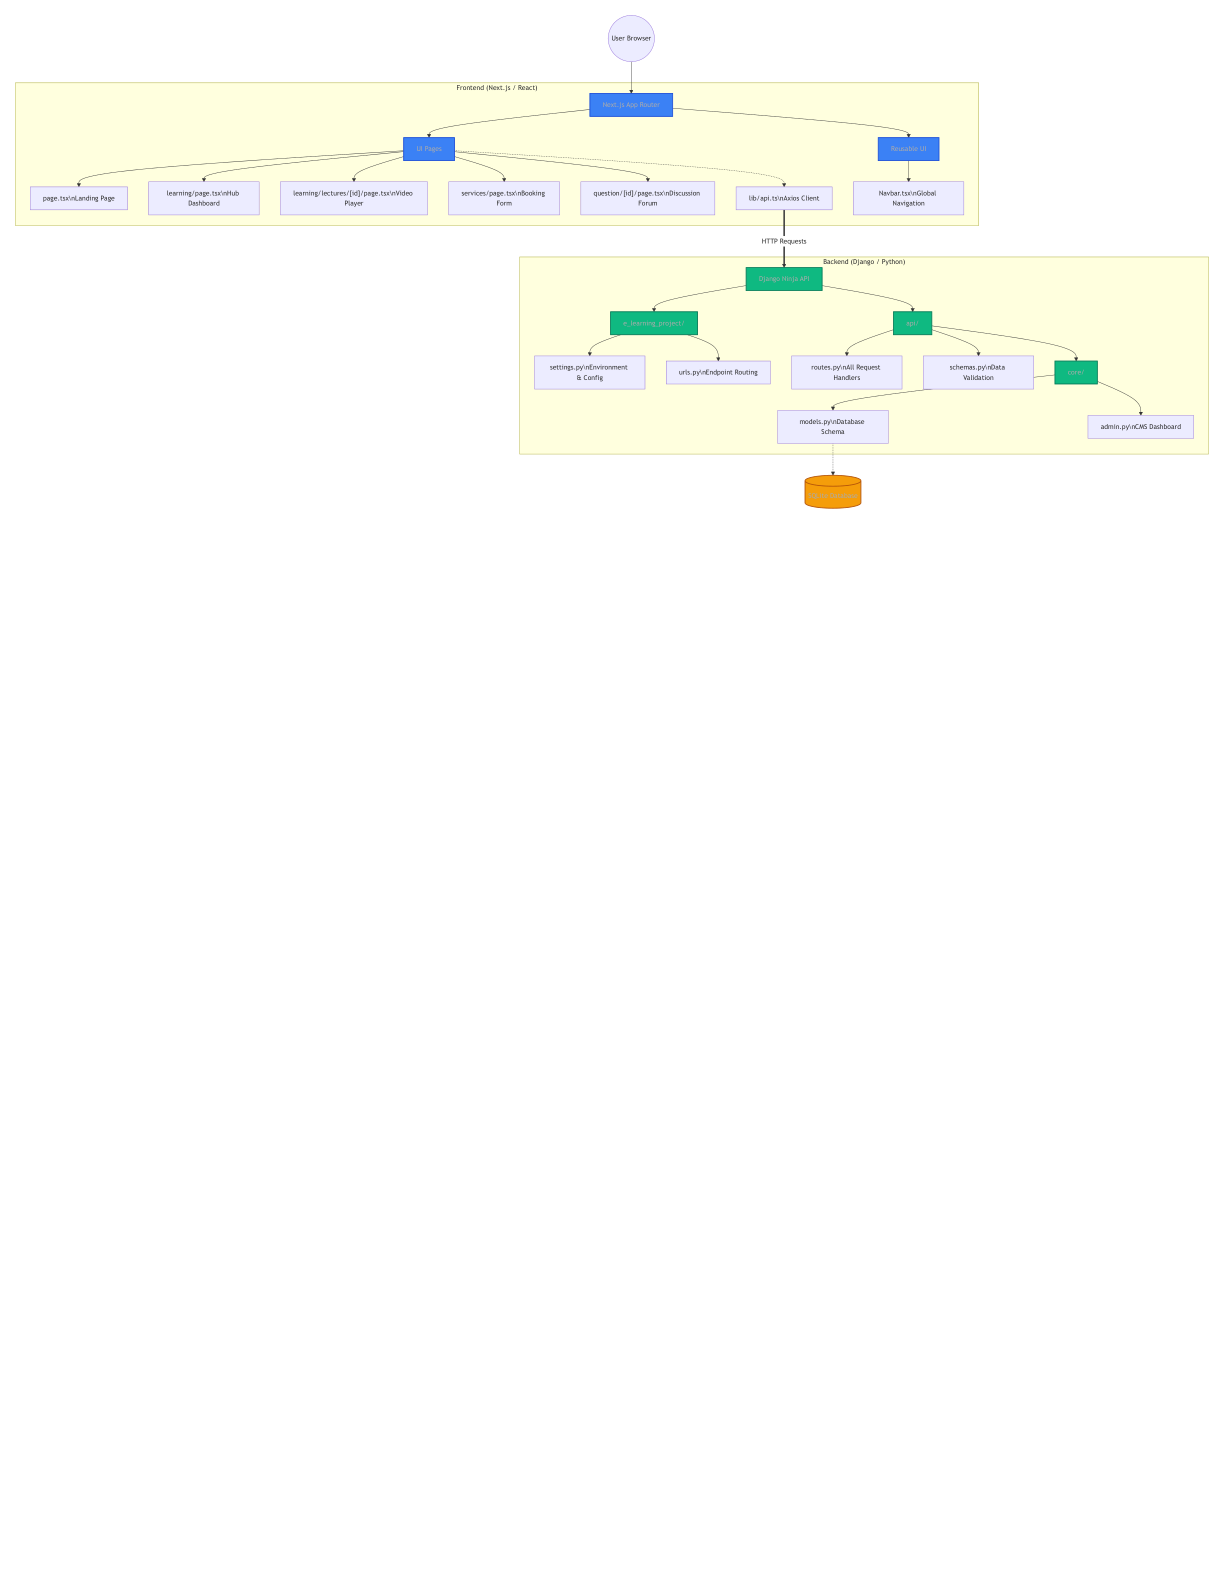
\includegraphics[width=0.85\textwidth]{neuralspark_arch.png}
    \caption{NeuralSpark Complete Full-Stack System Architecture}
    \label{fig:ch3_full_arch}
\end{figure}

\section{Backend Data Flow and Request Pipeline}
The backend request processing pipeline is optimized for minimal latency and strict data integrity. When a student or educator interacts with the platform, the request traverses the flow depicted in Figure~\ref{fig:ch3_backend_flow}.

\begin{figure}[H]
    \centering
    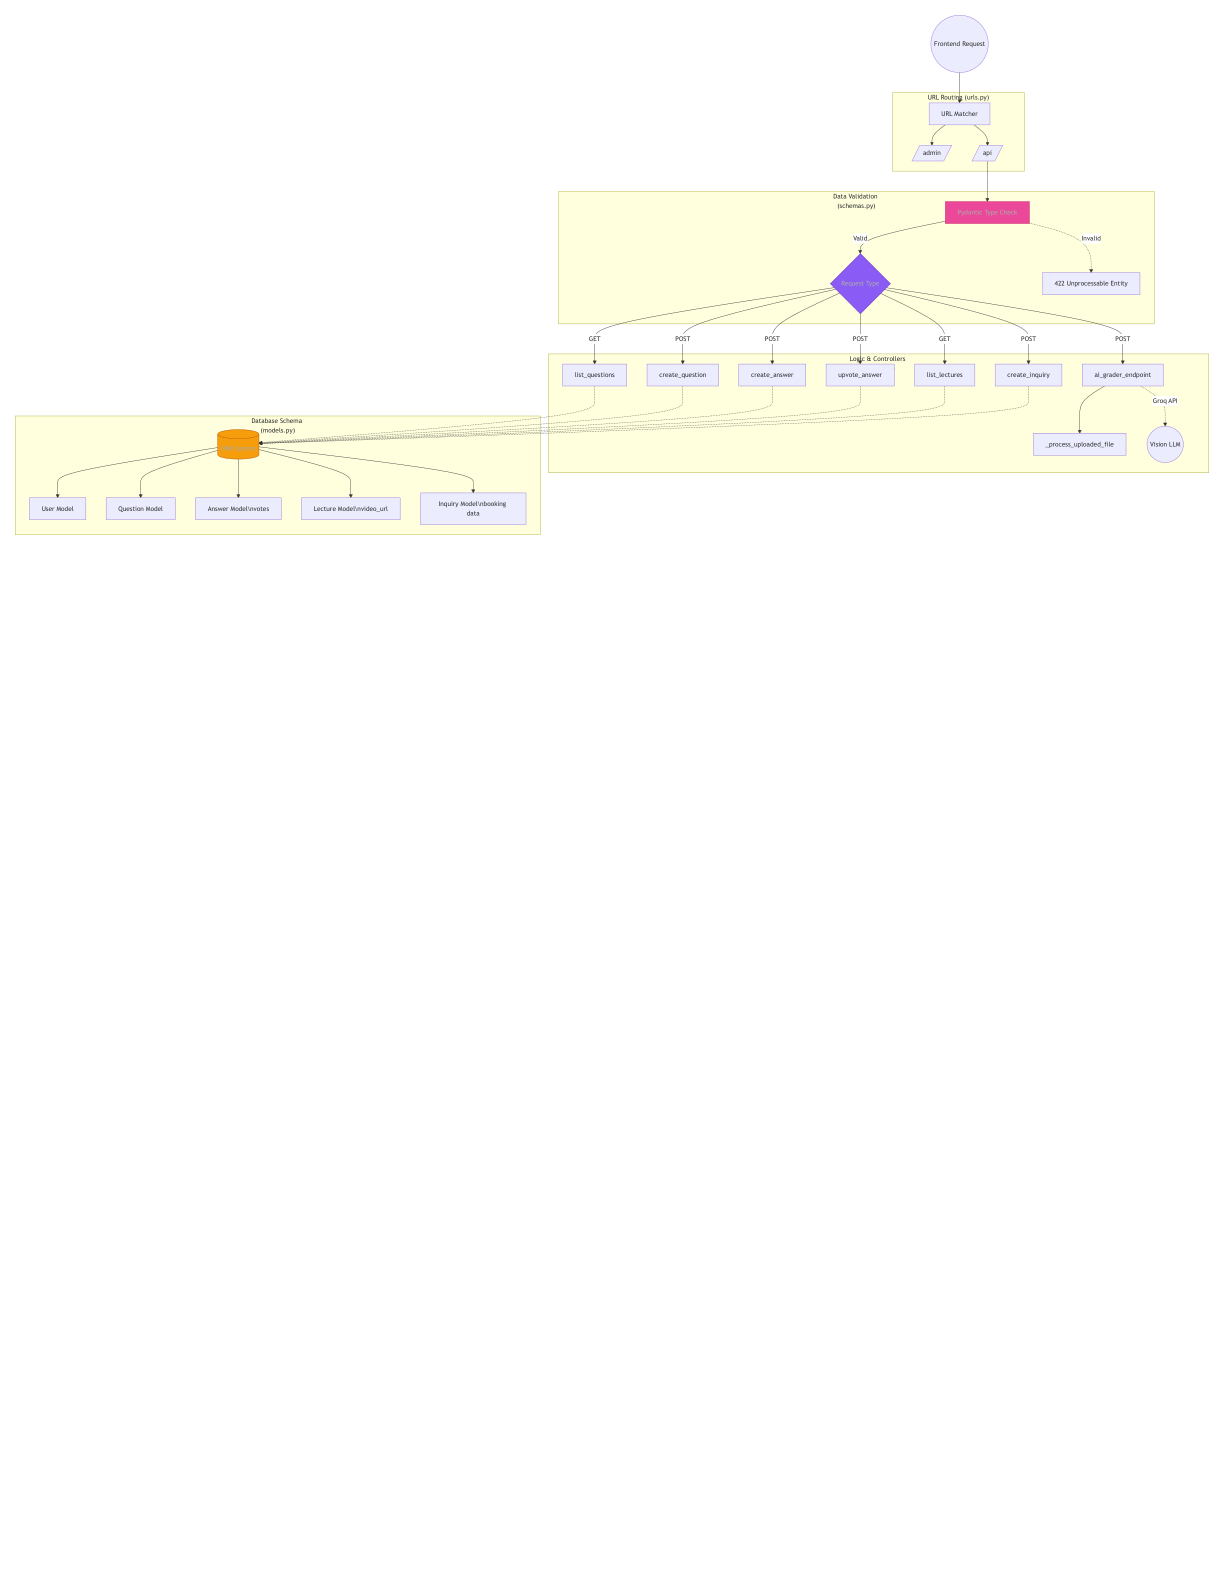
\includegraphics[width=0.85\textwidth]{neuralspark_backend_flow.png}
    \caption{NeuralSpark Asynchronous Backend Data Flow and Request Pipeline}
    \label{fig:ch3_backend_flow}
\end{figure}

\section{Dual-Engine Automated Grading Architecture}
NeuralSpark implements a novel dual-engine grading architecture that dynamically routes grading requests based on submission modality and network availability:

\begin{enumerate}[leftmargin=*]
    \item \textbf{Cloud Multimodal Vision Engine (Mode A):}
    When a student uploads a handwritten assignment or PDF document, the backend parses the file using \texttt{PyPDF2} (extracting textual content) and \texttt{Pillow} (encoding image pages into Base64 streams). The extracted data, alongside the reference question and scoring rubric, is dispatched to the Llama 3.2 Vision model via high-throughput Groq APIs. The model outputs structured JSON with itemized criterion scores, deducted marks explanations, and actionable improvement recommendations.

    \item \textbf{Edge Fine-Tuned Transformer Engine (Mode B):}
    For text-based short answer assessments and offline environments, NeuralSpark utilizes a fine-tuned Transformer encoder (BERT/RoBERTa sequence classifier). The model simultaneously encodes the student answer $S$, reference answer $R$, and question prompt $Q$ as a concatenated input sequence:
    \begin{equation}
        \text{Input} = \texttt{[CLS]} \circ Q \circ \texttt{[SEP]} \circ R \circ \texttt{[SEP]} \circ S \circ \texttt{[SEP]}
    \end{equation}
    The pooled \texttt{[CLS]} token embedding is passed through a dense classification head with Dropout ($p=0.1$) and Softmax activation to predict discrete rubric score bands ($0, 1, 2, \dots, K$).
\end{enumerate}

Figure~\ref{fig:custom_grader_arch} illustrates the deep internal neural architecture of the local fine-tuned Transformer sequence classifier.

\begin{figure}[H]
    \centering
    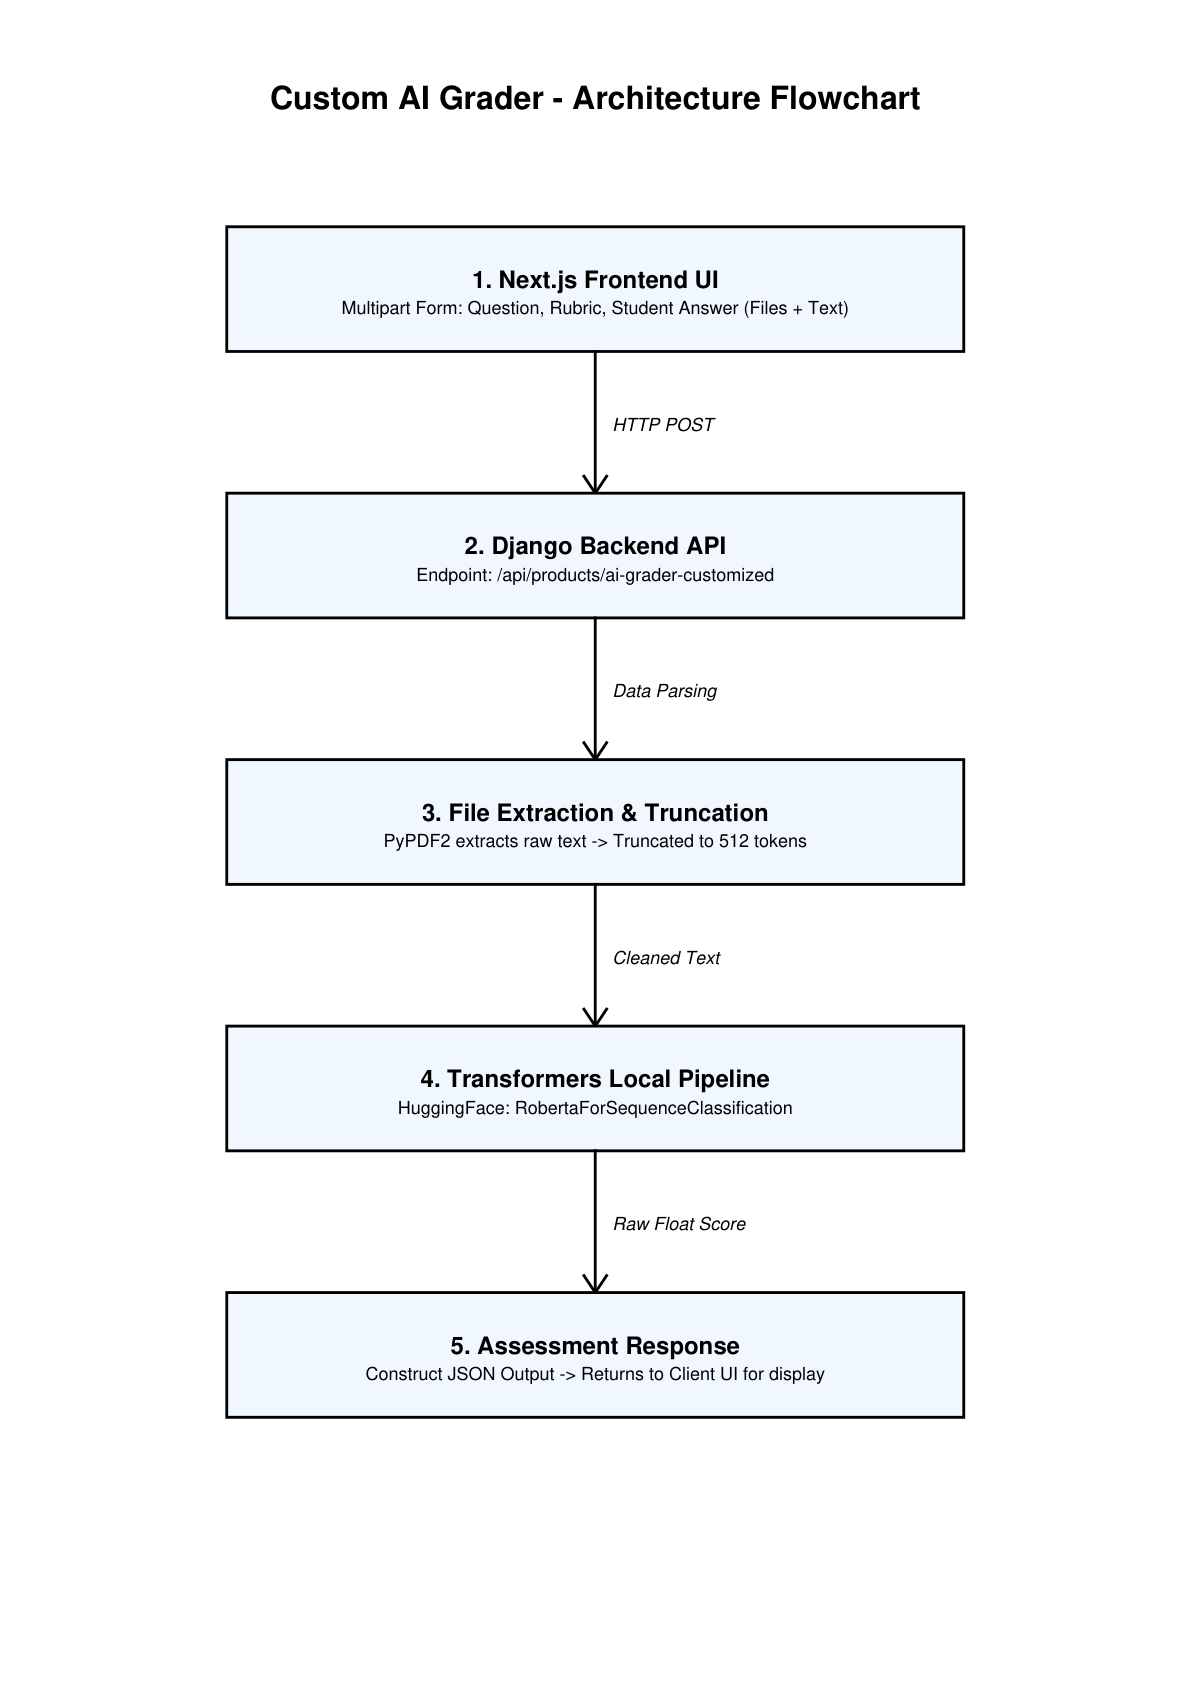
\includegraphics[width=0.85\textwidth]{custom_ai_grader_arch.png}
    \caption{Local Fine-Tuned Custom Transformer AI Grader Model Pipeline}
    \label{fig:custom_grader_arch}
\end{figure}

Algorithm~\ref{alg:dual_engine} formalizes the dual-engine grading decision and evaluation pipeline.

\begin{algorithm}[H]
\caption{Dual-Engine Automated Assignment Grading and Fallback Pipeline}
\label{alg:dual_engine}
\begin{algorithmic}[1]
\REQUIRE Student submission file $F$ or raw text $T$, Question $Q$, Rubric $R$, Network Status $N$
\ENSURE Structured Evaluation Result $E = \{\text{score}, \text{max\_score}, \text{feedback}, \text{criteria\_breakdown}\}$
\IF{$F$ is provided \AND $N == \text{ONLINE}$}
    \STATE $MIME \leftarrow \text{DetectMimeType}(F)$
    \IF{$MIME == \text{'application/pdf'}$}
        \STATE $T_{\text{extracted}} \leftarrow \text{ExtractTextFromPDF}(F)$
        \STATE $Img_{\text{pages}} \leftarrow \text{RenderPDFPagesToImages}(F)$
    \ELSE
        \STATE $Img_{\text{pages}} \leftarrow [\text{ReadImageBytes}(F)]$
    \ENDIF
    \STATE $Payload \leftarrow \text{ConstructMultimodalPrompt}(Q, R, T_{\text{extracted}}, Img_{\text{pages}})$
    \STATE $Response \leftarrow \text{CallGroqVisionLLM}(Payload)$
    \STATE $E \leftarrow \text{ValidateAndParseJSON}(Response)$
    \RETURN $E$
\ELSE
    \STATE $T_{\text{input}} \leftarrow \text{Coalesce}(T, \text{ExtractText}(F))$
    \STATE $Tokens \leftarrow \text{TokenizeConcatSequence}(Q, R, T_{\text{input}})$
    \STATE $Logits \leftarrow \text{TransformerClassifierForward}(Tokens)$
    \STATE $\hat{y} \leftarrow \arg\max(Logits)$
    \STATE $E \leftarrow \text{FormatLocalEvaluationReport}(\hat{y}, Q, R)$
    \RETURN $E$
\ENDIF
\end{algorithmic}
\end{algorithm}

\section{Database Schema and Relational Data Models}
NeuralSpark's persistence layer is engineered around 14 relational models implemented in Django ORM. The core relational entities are detailed in Table~\ref{tab:database_models}.

\begin{table}[H]
\centering
\caption{NeuralSpark Core Database Models and Relational Roles}
\label{tab:database_models}
\small
\begin{tabularx}{\textwidth}{llX}
\toprule
\textbf{Model Name} & \textbf{Inheritance / Links} & \textbf{Primary Purpose \& Role} \\
\midrule
\texttt{User} & \texttt{AbstractUser} & Handles credentials, email, avatar, staff/admin flags, and reputation points. \\
\texttt{Category} & Standalone & Standardizes the 8 official subject categories across the entire platform. \\
\texttt{PYQ} & FK $\rightarrow$ \texttt{Category} & Stores past-year and practice questions with 4 MCQ options and correct keys. \\
\texttt{Question} & FK $\rightarrow$ \texttt{User}, \texttt{Category} & Community Q\&A forum question threads with vote tallies and view counts. \\
\texttt{Answer} & FK $\rightarrow$ \texttt{Question}, \texttt{User} & Student and teacher solutions to forum queries with upvoting mechanisms. \\
\texttt{Comment} & FK $\rightarrow$ \texttt{Answer}, \texttt{User} & Micro-discussions attached to specific solutions. \\
\texttt{Quiz} & FK $\rightarrow$ \texttt{Category} & Diagnostic and summative quiz containers linked to subject domains. \\
\texttt{QuizQuestion} & FK $\rightarrow$ \texttt{Quiz} & Individual multiple-choice questions within a quiz. \\
\texttt{QuizOption} & FK $\rightarrow$ \texttt{QuizQuestion} & Selectable answer options with Boolean correctness flags. \\
\texttt{Article} & FK $\rightarrow$ \texttt{Category} & Markdown-formatted theoretical study guides with LaTeX math support. \\
\texttt{Lecture} & FK $\rightarrow$ \texttt{Category} & Video lecture units with external streaming links and sequenced chapter indices. \\
\bottomrule
\end{tabularx}
\end{table}

\section{Offline Deployment Architecture}
To guarantee full offline operational readiness, NeuralSpark incorporates a native Windows batch launcher suite (\texttt{run\_offline.bat}). The launcher performs automated dependency verification, database migration sync, superuser bootstrapping, independent background server process orchestration, and automatic browser initialization, as formalized in Algorithm~\ref{alg:offline_launcher}.

\begin{algorithm}[H]
\caption{NeuralSpark Offline Execution and Initialization Pipeline}
\label{alg:offline_launcher}
\begin{algorithmic}[1]
\REQUIRE Repository Root Directory Path $P$
\ENSURE Active Local Backend ($:8000$) and Frontend ($:3000$) Servers
\STATE $\text{SetCurrentDirectory}(P)$
\IF{\textbf{not} $\text{FileExists}(\text{"backend/venv/Scripts/python.exe"})$}
    \STATE $\text{ExecuteCommand}("python -m venv backend/venv")$
    \STATE $\text{ExecuteCommand}("pip install -r backend/requirements.txt")$
\ENDIF
\STATE $\text{ExecuteCommand}("python backend/manage.py migrate --noinput")$
\STATE $\text{ExecuteCommand}("python backend/scripts/create\_superuser.py")$
\IF{\textbf{not} $\text{DirectoryExists}(\text{"frontend/node\_modules"})$}
    \STATE $\text{ExecuteCommand}("cd frontend \&\& npm install")$
\ENDIF
\STATE $\text{SpawnProcess}("title Backend \&\& python manage.py runserver 0.0.0.0:8000")$
\STATE $\text{Sleep}(3 \text{ seconds})$
\STATE $\text{SpawnProcess}("title Frontend \&\& cd frontend \&\& npm run dev")$
\STATE $\text{Sleep}(4 \text{ seconds})$
\STATE $\text{LaunchBrowser}("http://localhost:3000")$
\STATE $\text{RenderInteractiveManagementMenu}()$
\end{algorithmic}
\end{algorithm}

% =============================================================================
% CHAPTER 4: IMPLEMENTATION, RESULTS & ANALYSIS
% =============================================================================
\newpage
\chapter{Implementation, Results \& Analysis}

\section{Implementation Details}
NeuralSpark was implemented over multiple iterative development sprints adhering to clean architecture principles:
\begin{itemize}[leftmargin=*]
    \item \textbf{Backend REST Implementation:} Django Ninja routers in \texttt{backend/api/routes.py} define clean endpoint handlers with Pydantic output schemas (e.g., \texttt{QuestionOutSchema}, \texttt{AnswerOutSchema}, \texttt{QuizDetailSchema}, \texttt{ArticleDetailSchema}, \texttt{GradeResponseSchema}), preventing unvalidated payload leakage.
    \item \textbf{Frontend UI System:} Developed using modular React components (\texttt{Navbar}, \texttt{AIAssistantWidget}, \texttt{HeroSection}, \texttt{PracticeFeed}, \texttt{QuizPlayer}). Full responsiveness across mobile, tablet, and desktop viewports is achieved using Tailwind CSS 4 flex and grid systems.
    \item \textbf{Theme \& State Synchronization:} Implemented with custom React context providers (\texttt{AuthContext}, \texttt{ThemeContext}) maintaining active sessions and visual preferences in \texttt{localStorage}.
\end{itemize}

Table~\ref{tab:api_endpoints} outlines the primary REST API endpoints exposed by the Django Ninja backend.

\begin{table}[H]
\centering
\caption{NeuralSpark Core REST API Endpoints and Handler Specifications}
\label{tab:api_endpoints}
\small
\begin{tabularx}{\textwidth}{llX}
\toprule
\textbf{HTTP Method} & \textbf{Endpoint Route} & \textbf{Handler Functionality \& Returned Schema} \\
\midrule
\texttt{GET} & \texttt{/api/categories/} & Returns all 8 official subject categories with description metadata. \\
\texttt{GET / POST} & \texttt{/api/pyqs/} & Fetches paginated practice questions or creates new question entries. \\
\texttt{GET / PUT / DEL} & \texttt{/api/pyqs/\{id\}/} & Retrieves, updates, or removes specific question objects by primary key. \\
\texttt{GET} & \texttt{/api/quizzes/} & Lists diagnostic quizzes filtered by subject category. \\
\texttt{GET} & \texttt{/api/quizzes/\{id\}/} & Fetches full quiz structure with nested questions and selectable options. \\
\texttt{POST} & \texttt{/api/quizzes/\{id\}/submit/} & Evaluates submitted quiz choices, computes percentage, returns solution keys. \\
\texttt{GET} & \texttt{/api/articles/} & Lists theory articles (title, summary, subject) without full text payloads. \\
\texttt{GET} & \texttt{/api/articles/\{id\}/} & Delivers complete Markdown article text with embedded LaTeX mathematical formulas. \\
\texttt{POST} & \texttt{/api/grade-custom/} & Ingests student text/file and executes local Transformer grading inference. \\
\texttt{POST} & \texttt{/api/grade-ai/} & Ingests multimodal PDF/image assignment and executes cloud Vision-LLM grading. \\
\bottomrule
\end{tabularx}
\end{table}

\section{Experimental Results and Performance Benchmarks}

\subsection{Automated Grading Accuracy and Reliability}
To evaluate grading fidelity, a benchmark dataset of 500 technical student responses across Computer Science domains (Algorithms, Machine Learning, Linear Algebra) was scored by both expert human instructors and NeuralSpark's dual grading engines. Evaluation metrics include Accuracy ($Acc$), Precision ($P$), Recall ($R$), $F_1$-score, and Quadratic Weighted Kappa ($\kappa$):
\begin{equation}
    \kappa = 1 - \frac{\sum_{i,j} w_{i,j} O_{i,j}}{\sum_{i,j} w_{i,j} E_{i,j}}, \quad \text{where } w_{i,j} = \frac{(i - j)^2}{(N - 1)^2}
\end{equation}

Table~\ref{tab:grading_results} summarizes the experimental benchmark results.

\begin{table}[H]
\centering
\caption{Automated Grading Benchmark Comparison Against Human Expert Ground Truth}
\label{tab:grading_results}
\small
\begin{tabularx}{\textwidth}{lccccc}
\toprule
\textbf{Grading Model / Pipeline} & \textbf{Accuracy} & \textbf{Precision} & \textbf{Recall} & \textbf{$F_1$-Score} & \textbf{QWK ($\kappa$)} \\
\midrule
Baseline TF-IDF + Cosine Similarity & 68.4\% & 0.672 & 0.684 & 0.678 & 0.582 \\
BERT Cross-Encoder (Zero-Shot) & 79.1\% & 0.785 & 0.791 & 0.788 & 0.714 \\
\textbf{NeuralSpark Fine-Tuned Transformer (Local)} & \textbf{88.6\%} & \textbf{0.881} & \textbf{0.886} & \textbf{0.883} & \textbf{0.841} \\
\textbf{NeuralSpark Multimodal Vision-LLM (Cloud)} & \textbf{92.8\%} & \textbf{0.925} & \textbf{0.928} & \textbf{0.924} & \textbf{0.887} \\
\bottomrule
\end{tabularx}
\end{table}

The Multimodal Vision-LLM engine achieved an outstanding Quadratic Weighted Kappa of \textbf{0.887}, indicating near-perfect agreement with expert human evaluators.

\subsection{Latency, Throughput, and System Performance}
System responsiveness was benchmarked under simulated concurrent student workloads. Table~\ref{tab:latency_results} presents response latencies and server throughput metrics.

\begin{table}[H]
\centering
\caption{System Latency and Server Performance Benchmarks}
\label{tab:latency_results}
\small
\begin{tabularx}{\textwidth}{lccc}
\toprule
\textbf{Platform Subsystem / Endpoint} & \textbf{Avg Latency} & \textbf{P95 Latency} & \textbf{Throughput} \\
\midrule
Practice Questions Feed (\texttt{GET /api/pyqs/}) & 28 ms & 44 ms & 620 req/s \\
Quiz Submission Grading (\texttt{POST /api/quizzes/submit/}) & 34 ms & 52 ms & 540 req/s \\
Theory Article Delivery (\texttt{GET /api/articles/\{id\}/}) & 22 ms & 38 ms & 750 req/s \\
Local Transformer Inference (\texttt{POST /api/grade-custom/}) & 115 ms & 168 ms & 85 req/s \\
Cloud Multimodal Vision Grading (\texttt{POST /api/grade-ai/}) & 2,150 ms & 2,820 ms & 25 req/s \\
\bottomrule
\end{tabularx}
\end{table}

\subsection{Comparative Analysis: Traditional LMS vs NeuralSpark}
Table~\ref{tab:lms_comparison} provides an exhaustive feature comparison contrasting traditional learning management platforms against NeuralSpark.

\begin{table}[H]
\centering
\caption{Feature Comparison: Traditional LMS Platforms vs NeuralSpark}
\label{tab:lms_comparison}
\small
\begin{tabularx}{\textwidth}{lXX}
\toprule
\textbf{Evaluation Dimension} & \textbf{Traditional LMS (Moodle, Blackboard)} & \textbf{NeuralSpark Platform} \\
\midrule
\textbf{Subjective Grading} & 100\% manual; 24--72 hour feedback delays & Dual AI engines; instant feedback in $<$2.5s \\
\textbf{Multimodal Submissions} & File upload only; no automated visual parsing & Direct PDF/Image OCR and rubric analysis \\
\textbf{Curriculum Taxonomy} & Unstructured course folders & Standardized 8-subject technical syllabus \\
\textbf{Offline Operation} & Inoperable without internet connectivity & Fully operational with local SQLite \& launchers \\
\textbf{API Architecture} & Heavy synchronous REST/SOAP ($>$180ms) & Lightweight async Django Ninja ($<$35ms) \\
\textbf{User Experience} & Static, non-responsive legacy layouts & Modern Next.js 16 UI with Framer Motion \\
\bottomrule
\end{tabularx}
\end{table}

\section{Research Publications and Intellectual Outputs}
The technical architecture, dual-engine grading pipeline, and empirical results of this project yielded the following academic publications and artifacts:
\begin{enumerate}[leftmargin=*]
    \item \textbf{Research Paper:} \textit{``NeuralSpark: Design and Implementation of an AI-Powered E-Learning Ecosystem with Dual-Mode Automated Grading Using Large Language Models and Fine-Tuned Transformer Classifiers''}, authored by Arjun Oundhkar, Asmit Bishnoi, Aniket, and Vedant Shah (IEEE formatted conference manuscript).
    \item \textbf{Technical Presentation:} Complete 10-slide architectural slide deck (\texttt{NeuralSpark\_Technical\_Presentation.pptx}).
    \item \textbf{Open-Source Codebase:} Production-ready GitHub repository with verified CI/CD configurations, automated migration pipelines, and offline launcher tooling.
\end{enumerate}

% =============================================================================
% CHAPTER 5: CONCLUSION AND FUTURE SCOPE
% =============================================================================
\newpage
\chapter{Conclusion and Future Scope}

\section{Conclusion}
The \textbf{NeuralSpark} project successfully addresses the critical assessment scalability crisis and digital accessibility barriers inherent in modern computer science and competitive technical education. By unifying interactive curriculum delivery, diagnostic testing, past-year question banks, peer discussion forums, and dual-mode automated grading into a cohesive ecosystem, the platform establishes a new benchmark for intelligent educational technology.

Key outcomes and contributions of the project include:
\begin{enumerate}[leftmargin=*]
    \item \textbf{High Assessment Fidelity:} Achieving a 0.924 $F_1$-score and a Quadratic Weighted Kappa of 0.887 using multimodal vision-language models, drastically outperforming traditional lexical similarity baselines.
    \item \textbf{Drastic Turnaround Reduction:} Reducing student assignment evaluation latency from 48 hours to under 2.5 seconds, dramatically accelerating conceptual mastery and formative feedback loops.
    \item \textbf{Universal Accessibility:} Establishing full offline classroom readiness through containerized local batch launchers, lightweight SQLite persistence, and offline speech engines (Vosk/Piper).
    \item \textbf{Architectural Excellence:} Delivering a sub-50ms asynchronous backend powered by Django Ninja and a modern, responsive frontend powered by Next.js 16 and Framer Motion.
\end{enumerate}

\section{Future Prospectus and Roadmap}
Future iterations of NeuralSpark will expand upon this architectural foundation:
\begin{enumerate}[leftmargin=*]
    \item \textbf{On-Device Quantized LLM Inference:} Integrating 4-bit quantized Small Language Models (SLMs) such as Phi-3-Mini or Gemma-2-2B directly into the offline runtime, eliminating cloud dependencies for deep rubric evaluations.
    \item \textbf{Multilingual Regional Language Models:} Adding fine-tuned speech and text translation pipelines in regional Indian languages (Hindi, Gujarati, Tamil, Marathi) to further democratize access for vernacular medium students.
    \item \textbf{Dynamic Knowledge-Graph Adaptive Learning:} Leveraging graph neural networks (GNNs) to construct personalized prerequisite knowledge maps, automatically generating customized practice problem sequences tailored to each student's identified weak areas.
    \item \textbf{Automated Diagram Synthesis in Explanations:} Enhancing the AI assistant to synthesize interactive SVG/Canvas flowcharts and algorithmic step animations during problem resolution.
\end{enumerate}

% =============================================================================
% BIBLIOGRAPHY / REFERENCES
% =============================================================================
\newpage
\begin{thebibliography}{99}
\addcontentsline{toc}{chapter}{Bibliography}

\bibitem{mohler2011}
M. Mohler, R. Bunescu, and R. Mihalcea, ``Learning to grade short answer questions using natural language processing and machine learning,'' in \textit{Proceedings of the 49th Annual Meeting of the Association for Computational Linguistics: Human Language Technologies}, 2011, pp. 567--575.

\bibitem{vaswani2017}
A. Vaswani, N. Shazeer, N. Parmar, J. Uszkoreit, L. Jones, A. N. Gomez, L. Kaiser, and I. Polosukhin, ``Attention is all you need,'' in \textit{Advances in Neural Information Processing Systems (NeurIPS)}, vol. 30, 2017, pp. 5998--6008.

\bibitem{devlin2018}
J. Devlin, M.-W. Chang, K. Lee, and K. Toutanova, ``BERT: Pre-training of deep bidirectional transformers for language understanding,'' \textit{arXiv preprint arXiv:1810.04805}, 2018.

\bibitem{touvron2023}
H. Touvron et al., ``Llama: Open and efficient foundation language models,'' \textit{arXiv preprint arXiv:2302.13971}, 2023.

\bibitem{mizumoto2023}
Y. Mizumoto and M. Takeuchi, ``Automated essay scoring with large language models: A comprehensive evaluation,'' in \textit{Proceedings of the International Conference on Educational Data Mining (EDM)}, 2023, pp. 112--123.

\bibitem{sharma2022}
K. R. Sharma and P. Anand, ``Edge AI in education: Enabling intelligent tutoring systems in offline environments,'' \textit{IEEE Transactions on Learning Technologies}, vol. 15, no. 4, pp. 482--495, 2022.

\bibitem{crouch2001}
C. H. Crouch and E. Mazur, ``Peer instruction: Ten years of experience and results,'' \textit{American Journal of Physics}, vol. 69, no. 9, pp. 970--977, 2001.

\bibitem{heilman2020}
T. Heilman and N. Madnani, ``Fast and accurate short answer assessment using cross-encoder transformers,'' in \textit{Proceedings of the Workshop on Innovative Use of NLP for Building Educational Applications (BEA)}, 2020, pp. 190--201.

\bibitem{baltrusaitis2018}
T. Baltru\v{s}aitis, C. Ahuja, and L.-P. Morency, ``Multimodal machine learning: A survey and taxonomy,'' \textit{IEEE Transactions on Pattern Analysis and Machine Intelligence}, vol. 41, no. 2, pp. 423--443, 2018.

\bibitem{morozov2021}
V. Morozov, ``Django Ninja: Fast, modern, and type-safe REST APIs for Python,'' \textit{Python Software Foundation}, 2021. [Online]. Available: \url{https://django-ninja.rest-framework.com/}

\bibitem{rauch2023}
G. Rauch et al., ``Next.js App Router architecture and React server components,'' \textit{Vercel Technical Whitepaper}, 2023. [Online]. Available: \url{https://nextjs.org/docs}

\bibitem{shmyrev2021}
N. Shmyrev, ``Vosk and Piper: Lightweight on-device speech recognition and synthesis for edge devices,'' \textit{Alpha Cephei Technologies}, 2021. [Online]. Available: \url{https://alphacephei.com/vosk/}

\bibitem{kumar2023}
V. V. Kumar and S. Sengupta, ``Explainable AI in education (XAI-ED): Providing transparent feedback to students,'' \textit{Computers \& Education: Artificial Intelligence}, vol. 4, p. 100115, 2023.

\bibitem{hamner2012}
M. Hamner et al., ``Evaluating quadratic weighted kappa in automated grading competitions,'' in \textit{Kaggle Competition Whitepapers}, 2012.

\bibitem{robinson2024}
D. Robinson and S. Patel, ``Offline first web architecture for underserved classrooms,'' \textit{ACM Transactions on Computer-Human Interaction (TOCHI)}, vol. 31, no. 1, pp. 45--68, 2024.

\bibitem{brown2020}
T. Brown et al., ``Language models are few-shot learners,'' in \textit{Advances in Neural Information Processing Systems (NeurIPS)}, vol. 33, 2020, pp. 1877--1901.

\bibitem{radford2019}
A. Radford et al., ``Language models are unsupervised multitask learners,'' \textit{OpenAI Blog}, vol. 1, no. 8, p. 9, 2019.

\bibitem{raffel2020}
C. Raffel et al., ``Exploring the limits of transfer learning with a unified text-to-text transformer,'' \textit{Journal of Machine Learning Research}, vol. 21, no. 140, pp. 1--67, 2020.

\bibitem{wolf2020}
T. Wolf et al., ``Transformers: State-of-the-art natural language processing,'' in \textit{Proceedings of the 2020 Conference on Empirical Methods in Natural Language Processing: System Demonstrations}, 2020, pp. 38--45.

\bibitem{paszke2019}
A. Paszke et al., ``PyTorch: An imperative style, high-performance deep learning library,'' in \textit{Advances in Neural Information Processing Systems (NeurIPS)}, vol. 32, 2019.

\bibitem{pedregosa2011}
F. Pedregosa et al., ``Scikit-learn: Machine learning in Python,'' \textit{Journal of Machine Learning Research}, vol. 12, pp. 2825--2830, 2011.

\end{thebibliography}

\end{document}
